\documentclass{article}

\usepackage[utf8]{inputenc}
\usepackage[T1]{fontenc}
\usepackage{amsmath}
\usepackage{amsfonts}
\usepackage{amssymb}
\usepackage[version=4]{mhchem}
\usepackage{stmaryrd}
\usepackage{bbold}
\usepackage{float}
\usepackage{graphicx}
\usepackage{adjustbox}
\usepackage{hyperref}  % For clickable links in TOC
\usepackage{tocloft}   % For TOC formatting
\usepackage{geometry}  % For margins
\usepackage{titlesec}  % For section formatting
\usepackage[english]{babel}

\newtheorem{definition}{Definition}[section]

% Retrieves visuals 
% visuals

% expected result blue boxes
\usepackage[most]{tcolorbox}
\newtcolorbox{expectedresultsbox}{colback=blue!2!white, colframe=blue!75!black, arc=4mm, boxrule=0.5mm}

% intro black box
\newtcolorbox{GTbox}[1][]{%
  enhanced,
  colback=white,
  colframe=blue,
  arc=4mm,                % rounded corners
  fonttitle=\bfseries,
  title={\large Solving with Grim-trigger},
  center title,
  #1
}

\newtcolorbox{Proof}[1][]{%
  enhanced,
  colback=white,
  colframe=blue,
  arc=4mm,                % rounded corners
  fonttitle=\bfseries,
  title={\large Proof},
  center title,
  #1
}

\newtcolorbox{simplebox}[1]{  
  title=#1,               % Title from argument  
  colback=blue!10,        % Light blue background  
  colframe=blue!70!black, % Dark blue frame  
  fonttitle=\bfseries,    % Bold title  
  boxrule=0pt,            % No frame around the text area  
  toprule=2mm,            % Thick rule at the top (blue band)  
  enhanced,               % Required for shadow  
  drop shadow             % Simple shadow with default settings  
}  

% Customize section formatting
\titleformat{\section}
  {\normalfont\Large\bfseries}
  {}
  {0pt}
  {\thesection\quad\rule{\linewidth}{0.4pt}\vspace{0.5em}\newline}
{\normalfont\Large\bfseries}


\title{Microeconomics 2 : Game Theory}
\author{Romain Fernex}
\date{January 2025}

\begin{document}

\maketitle
\tableofcontents
\newpage

\section{Session 1 : Pure strategies}
\subsection{Definitions and theorems}
\begin{itemize}
    \item Strategy profile : collection of strategies (one for each player) that specifies how each player will act in every situation $(s_1,s_2,....s_N)$, with N the nb of players
    \item Strategy space : set that contains all strategies available to the player (regardless of whether they are rational or not)
    \item Rationalizability : set of rationalizable strategies is $\bigcap_{i=1}^\infty S_i^k $
        \subitem - strategy is rationalizable if it is a best response to beliefs that are themselves consistent with the rationality of others
        \subitem - This concept is weaker than Nash Equilibrium because it does not require beliefs to be correct, only consistent with rationality. It captures strategic reasoning without assuming perfect foresight.
    \item Best response set ($BR_i(s_{-i})$) of player i to strat $s_-i$ = $argmax_{s_i\in S_i} u_i(s_i,s_{-i})$
    \item Correctness of a players belief : A player's belief is correct if he plays by that belief (strategies match beliefs)
    \item Nash Equilibrium : a strategy profile is a NE of G if $\forall i$ and $\forall s_i' \in S_i$ we have $u_i(s_i^{NE},S_{-i}^{NE})\geq u_i(s_i',S_{-i}^{NE}) $
        \subitem - formal definition : best response to my opponents best response ! (look for reciprocity of best responses)
        \subitem - situation that neither player would wish to deviate from unilaterally (either you both deviate or you don't)
\end{itemize}

\subsection{Methods and Tricks}

\subsubsection{n°1 : Identifying the strict dominance of a strategy for a given player}
\begin{itemize}
    \item visual method : for player 2 : compare right-hand terms from the column of interest to those in all other columns, if they are strictly superior to all of them (pairwise comparisons) then this strategy is dominant
        \subitem - For player 1 : similar approach but reasons in rows and consider the left-hand terms
\end{itemize}

\subsubsection{n°2 : Iterated strict dominance method}
\begin{itemize}
    \item $\forall k \in {1,..,N} $, define $S_i{k+1} = $
    \item $s_i \in S_i^k \mid \not\exists s_i' \in S_i^k$ with $ u_i(s_i', s_{-i}) > u_i(s_i, s_{-i}) $ for all $ s_{-i} \in S_{-i}^k$
    \item a dominant strategy exists if $\bigcap_{i=1}^\infty S_i^k $ is a singleton
    \item in practice : 
        \subitem - Look at columns : if a column dominates another, eliminate the dominated column
        \subitem - Now look at remaining rows (the other player) : if a row dominates another then remove the dominated row
        \subitem - go back to square one and repeat the cycle as long as necessary until you can't find a dominated row/column
\end{itemize}

\subsubsection{n°3 : Finding the rationalizable set}
\begin{itemize}
    \item just use the iterated strict dominance method, the set obtained will be the same as the rationalizable set 
\end{itemize}

\subsubsection{n°4 : Finding the Nash Equilibrias(classic)}
\begin{itemize}
    \item determine the rationalizable set 
    \item Look at each player separately and write down their best responses to each possible action of the opposite player
    \item Now find the best responses to the best responses you determined previously $\rightarrow$ if it is a subset of the rationalizable set then this subset is the set of Nash Equilibrias (IMPORTANT : iterated dominant strategy $\rightarrow$ Nash equilibria but not reverse)
    \item non existence of NEs : 
        \subitem - in pure strategies you conclude there are no Nash equilibria when: For every profile of pure strategies, at least one player can unilaterally switch his or her strategy to improve the payoff. OR There is no pair (or set, in games with more players) of actions such that each player's action is the best response to the other players’ actions.
\end{itemize}

\subsubsection{n°5 : Finding Nash Equilibrias with N players in a simultaneous game with cooperation}
\begin{itemize}
    \item Find situations that NO players would wish to deviate from (calculate cost/benefit of deviating individually for each player starting from a given situation $\rightarrow$ if it results in a loss for both then this is a NE)
    \item alt : circle Best responses for each line / column $\rightarrow$ if a strategy is the best response for both players it is a NE 
\end{itemize}

\subsubsection{n°6 : Solving Cournot Competition problems}
\begin{itemize}
    \item Define the formula for profits for each player ($\pi_i$)
\begin{equation}
    ex : \pi_i=P(Q)q_i-cq_i \text{ with P(Q) the inverse demand function for aggregate quantities}
\end{equation}
    \item Find the best response of player i to $p_j$ ($q_j$) : Derive the FOC for player i wrt to $p_i$ (or $q_i$ depending on the set up) to maximize $\pi_i$ as a function of $p_j$ (respectively $q_j$)
    \item Do the same with for player j to find $BR(q_i)$ (respectively $BR(p_i)$)
    \item solving methods : 
        \subitem - graphically (if 1x1) : by representing the set of best responses for each player $\rightarrow$ the nash equilibrium is the pair $(q_i,q_j)$ where the curves cross each others
        \subitem - iterated strict dominance : same as described earlier 
\end{itemize}

\section{Session 2 : Mixed strategies}

\subsection{Definitions}
\begin{itemize}
    \item Mixed strategy : present in games in which players randomize over actions. A strategy is then defined by the probability you place on each action, it is a distribution on $S_i$ for player i.\\
    Mathematical definition of a mixed strategy $\sigma_i$ :
    \begin{equation}
        u_i(\sigma_i,\sigma_{-i}) = \sum_{s_i, s_i} u_i(s_i, s_{-i})\sigma_i(s_i)\sigma{-i}(s_{-i})
    \end{equation}
$s_i$ is a pure strategy playable by player i ($\in S_i$ the set of pure strategies playable by player 1)
    \item MSNE : a mixed strategy profile is a MSNE of G if :
    \begin{equation}
\forall i, \forall \sigma_i\in\sum_i ,\hspace{1em} u_i(\sigma_i^{NE},\sigma_{-i}^{NE}) \geq u_i(\sigma_i',\sigma_{-i}^{NE})
    \end{equation}
    \item A MSNE exists when : 
        \begin{enumerate}
            \item a player cannot unilaterally deviate to increase his expected utility (for instance, can't assigne positive probabilities to another pure strategy, or cannot change the probabilities assigned to the strategies considered)
            \item player i must be indifferent between every pure strategy $s_i$ played with strictly positive probabilities in $\sigma_i$ (otherwise he would go for a degenerate lottery in favor of the most favorable strategies)
            \begin{equation}
                u_i(s_i,\sigma_{-i}^{NE}) = u_i(s_i',\sigma_{-i}^{NE})
            \end{equation}
        \end{enumerate}
\end{itemize}

\subsection{Properties}
\begin{itemize}
    \item existence of a NE : in a game with a finite nb of players and actions there will always exist a NE
\end{itemize}

\subsection{Methods}

\subsubsection{Solving for mixed NEs}
\begin{itemize}
    \item step 1 : assign probabilities to each option for each player (be mindful of which option you ascribe positive probabilities to)
    \item step 2 : compute expected payoffs for each options with a positive probability for each player
    \item step 3 : use the indifference condition to find equilibrium probabilities 
    \item \textbf{WARNING : }when a question asks you to find all the mixed strategy NE, you should include the pure strategy NE in your answer as a pure strategy is nothing but a special case of mixed strategy. 
\end{itemize}

\subsubsection{Lotteries and payoffs}
\begin{itemize}
    \item if you know the payoff for a strategy is equivalent to the expected payoff of a given lottery, you can compute this expected payoff and assume it is the payoff of the strategy in question
\end{itemize}

\subsubsection{Reducing the number of strategies with positive probabilities}
\begin{itemize}
    \item SEE WITH JUAN
\end{itemize}






\section{Session 3 : sequential games}

\subsection{Definitions}
\begin{itemize}
    \item pure strategy (for a given player i) : $s_i : H_i \rightarrow A_i | s_i(x)\in A(x)$ for each $x\in H_i$ 
    \begin{itemize}
        \item $H_i$ : set of nodes at which player i moves
        \item $A(x)$ : set of playable strategies for player i when faced with decision node x 
        \item $s_i(x)$ : strategy played by player i at node x
    \end{itemize}
    \item non credible threats:  a threat that can be considered as not rationally enforcable as it would result in a loss of utility for the one carrying out the punishment
    \item subgame : for G an extensive form games with nodes in set X, a subgame G' of G is a subset $Y\subset X$ with a single \textbf{non-terminal} node $x\in X$ and all its successors. It includes : 
    \begin{enumerate}
        \item A single non-terminal node x in X. This is a node where decisions are still made, not a final outcome.
        \item A subset Y that includes this node x and all its successors. "Successors" here means every node that can be reached from x following the paths of the game (including subsequent decision nodes, chance nodes, and terminal nodes).
    \end{enumerate}
    \item subgame perfect Nash equilibrium : 
    \begin{itemize}
        \item goal : eliminate non-credible threats
        \item A strategy profile is subgame perfect if it induces a Nash equilibrium in every subgame 
    \item one-stage deviation principle : $s_i$ is SP if $\forall i,t,a_i$ $U(s_i) \geq U(s_{-i},a'_i) $ with $a_i \in A_i(t)$ any alternative action that can be taken at any period t by player i
    \begin{itemize}
        \item check for potential deviations at every single stage
    \end{itemize}
    \end{itemize}
\end{itemize}

\subsection{Methods and tricks }
\subsubsection{Finding the subgame perfect equilibrias using backwards induction}
\begin{itemize}
    \item start from the end (nodes right before the terminal nodes)
    \item determine the optimal choice of the player playing last
    \item based on this optimal choice, find the optimal of the player playing at the previous node $\rightarrow$ keep doing that until you find the only viable pure strategies that are left
\end{itemize}
\begin{figure}[htbp]
  \centering
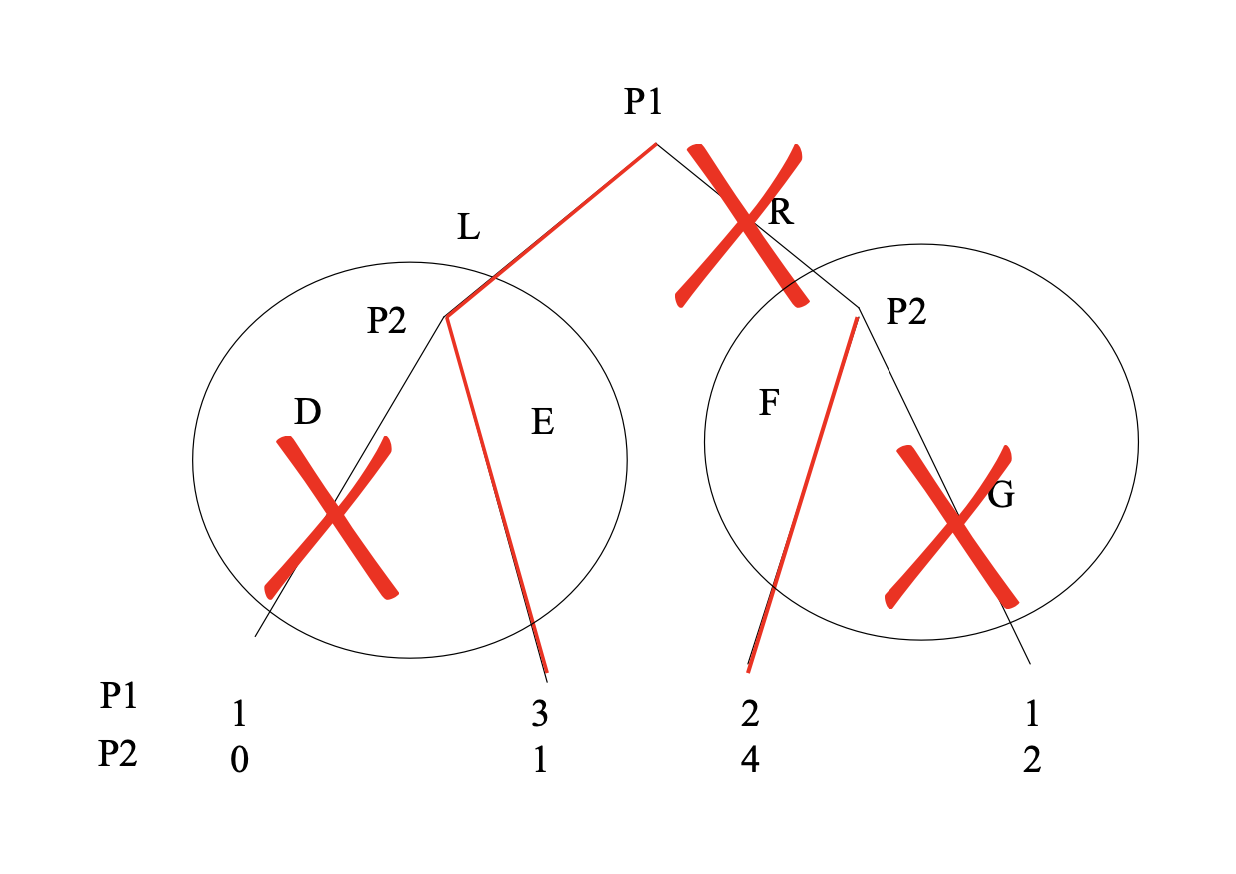
\includegraphics[width=0.7\linewidth]{tree_subgame_perfect.png} % adjust the width as needed
  \caption{Example of a subgame perfect NE}
  \label{fig: Finding a subgame perfect NE}
\end{figure}

\subsubsection{Stackelberg Quantity competition}
\begin{itemize}
    \item  Set-up : firm 1 chooses $q_1$ to optimize its profits. Then firm 2 chooses $q_2$ based on the chosen $q_1$  to optimize its profits. 
    \item Characteristics : 
    \begin{itemize}
        \item non-credible threat from player 2 of playing $q_2$ such that neither player get any profit
        \item multiple equilibrias possible
    \end{itemize}
    \item how to solve ? 
    \begin{enumerate}
        \item compute best response quantity $BR(q_1) = q^*_2$ assuming $q_1$ known
        \item compute optimal quantity for player 1 as a function of $BR(q_1)$
    \end{enumerate}
\end{itemize}

\subsubsection{Preemptive action - entry deterrence game}
\begin{itemize}
    \item Introduce a new choice ahead of the existing choice to change the the subgame perfect NE (and thus the terminal outcome)
    \item Solving the entry deterrence game : 
    \begin{enumerate}
        \item Follow the same steps as with the classic Stackelberg quantity competition game
        \item Express $q_1^*$ as a function of f (entry tax) and replace it in the profit function
        \item Maximize $\pi_1$ with respect to f to find optimal entry tax that player 1 should implement
    \end{enumerate}
\end{itemize}

\subsubsection{Rubinstein bargaining model}
\begin{itemize}
    \item use the one stage deviation principle to find the unique SPNE
    \item only need to check existence of a profitable deviation when : 
    \begin{enumerate}
        \item player 1 makes an offer (consider deviation when player 2 refuses the offer) --> shows payoff is at most as good as the one she would have accepted without deviating
        \item player 2 makes an offer (same principle but with player 1)
    \end{enumerate}
\end{itemize}


\section{Session 4 : repeated games}
    
\subsection{Definitions}
\begin{itemize}
    \item stage game : game that is repeated 
    \item correlated equilibrium : 
    \item set of feasible payoff vectors (\textcolor{blue}{blue line}) : a payoff vector v is feasible if there exist action profiles $(a_1,...)$ and non negative weights $\lambda_1, ...$ with $\sum\lambda_k=1$ such $\forall i$, $v_i = \sum \lambda_ku_i(a_k)$
        \begin{itemize}
            \item in other words : Feasible payoff vectors represent outcomes that are possible or can be "realized" by appropriately randomizing over the available action profiles (set of outcomes players might be able to enforce or agree upon)
        \end{itemize}
        \item set of strictly individually rational payoff vectors (\textcolor{red}{red line}) : a payoff vector v is S.I.R if $\forall i, v_i > \min_{\sigma_{-i}\in\sum_{-i}}[\max_{\sigma_i\in\sum_{i}}u_i(\sigma_i,\sigma_{-i})] = \underline{v_i}$
        \begin{itemize}
            \item in other words : A payoff vector v is strictly individually rational if each player's payoff is strictly greater than their min-max payoff.
            \item min-max payoff : The min-max payoff for a player is the minimum payoff they can guarantee themselves regardless of what other players do.  (worst punishment player i's opponents can coordinate on imposing)
        
        \end{itemize}
    \begin{figure}[H]
  \centering
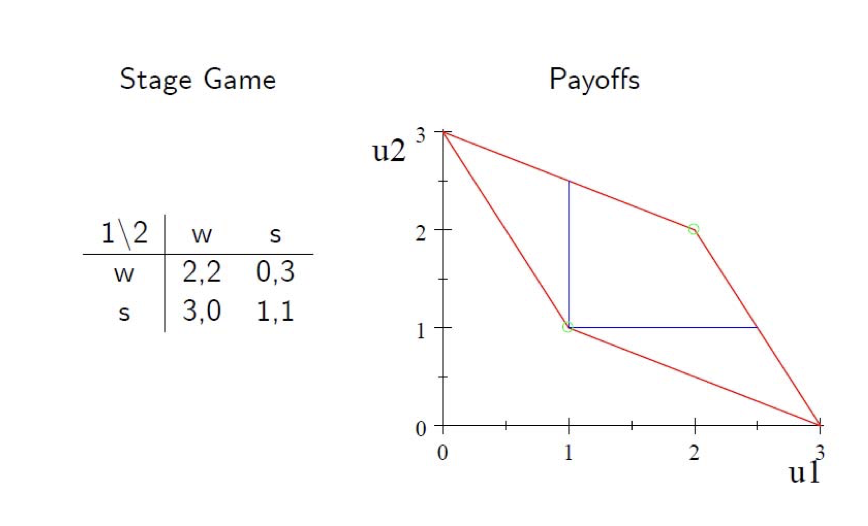
\includegraphics[width=0.7\linewidth]{Folk-game.png} % adjust the width as needed
  \caption{Example of game with payoff sets}
  \label{fig: Game example with payoff sets}
\end{figure}
    \item  critical discount factor: The critical discount factor for player for player i is the lowest value of $\delta_i$ such that when $\delta_i \geq \underline{\delta_i}$, the strategy profile that yields payoff $v_i$ for player i is NE. n other words, if players value future payoffs at least as much as this threshold value, the threat of future punishment (or loss of cooperative gains) is sufficient to deter unilateral deviation, making the equilibrium sustainable.
\end{itemize}

\subsection{Repeated Finite game }

\subsubsection{Properties}
\begin{itemize}
    \item Proposition : if a stage game has a unique NE, then players will play the NE strategy of the stage game in every period !
\end{itemize}

\subsubsection{Solving method}
\begin{itemize}
    \item solving method : use backwards induction
    \item n°1 : if a stage game has a unique NE, then unique SPNE in a finite repetition is such that players play the NE strategy of the stage game in every period
    \begin{enumerate}
        \item Knowing that every player will play the stage game’s NE in the last period, the same logic applies in the second-to-last period because any deviation is not rewarded in the final period. This logic is applied period by period backward to the first period.
    \end{enumerate}
\end{itemize}

\subsection{Repeated Infinite game}

\subsubsection{Properties}
\begin{itemize}
    \item For a single Strategy, there are many possible SPNE (play C:C at every period, D:D etc..)
    \item Whenever we finnd a condition under which a set of strategies forms a SPNE of an infnitely repeated game it is always going to be of the type : $\delta \geq \bar{\delta}$
    \begin{itemize}
        \item Why ? : player care about the future and fear punishments following a deviation
        \item implication : anything can be an equilibrium if $\delta$ high enough
        \item limit : Folk's theorem
    \end{itemize}
    \item Folk theorem : G a simultaneous move game, $A_1,A_2,..A_I$ the action sets, $u_1,u_2..$ the payoff functions 
    \begin{itemize}
        \item Version 1 : for any feasible$\cap$ S.I.R payoff vector v, $\exists\delta<1|\forall\delta\geq\underline{\delta}, \exists\sigma^*$ a NE of $G(\delta)$ with payoff v
\begin{Proof}
    \begin{enumerate}
        \item take a game where each player i adopts the following strategy : keep cooperating (play $a_i$) if 1)everyone cooperated so far, 2)more than one player deviated before (in other words, if a player deviates alone he will be punished)
        \item normalize payoff by $(1-\delta_i)$ to get rid of infinite sums
        \item the payoff resulting from deviation is : 
\begin{equation}
    NPV (deviation) = \underbrace{(1-\underline{\delta_i})max_{a_i}g_i(a_i',a_{-i})}_{\text{payoff from deviation}}+\underbrace{\underline{\delta_iv_i}}_{NPV (post -punishment)}
\end{equation}
        \item find the critical discount factor $\underline{\delta}_i$ by solving : $NPV(deviation)=v_i$
    \end{enumerate}
\end{Proof}
        \item version 2 : Let $\alpha^*$ be a static equilibrium of stage game with payoff e, then $\forall v\in V$ with $v_i>e_i$, for all players i,$\exists \underline{\delta}<1|\forall \delta\geq\underline{\delta},\exists$ a SPNE of $G(\delta)$ with payoff v.
    \end{itemize}
    \begin{enumerate}
        \item
    \end{enumerate}
\end{itemize}

\subsubsection{Check if a strategy is SPNE in a repeated infinite game}
\begin{itemize}
    \item decide on the equilibrium you are considering
    \item define the overall strategy that both players will be following throughout the whole game (grim trigger, tit for tat..)
    \item consider all possible subgames/configurations (for instance : one player played C before, no player ever played C before...)
    \item for each of these configuration compare the expected payoff of deviating at this round (and this round only : one stage deviation) to that of not deviating. 
    \item check if there exists conditions on delta such that the strategy you adopted is NE every subgame (never profitable to deviate from that strategy)
\end{itemize}

\subsubsection{Grim-trigger strategy}
\begin{itemize}
    \item if someone deviates from the agreement, it triggers a common punishment forever (classic perception of the prisoner's game in infinite time)
    \item limit : works only if players care enough for the future ($\delta$ high enough)
\end{itemize}

\subsubsection{Price Collusion game}
\begin{itemize}
    \item set up : 
    \begin{enumerate}
        \item $N\geq 2$ firms, with the same constant marginal cost c, choose prices at each stage
        \item profits of a firm : $\pi(p) = (p-c)Q(p)$
        \item custmer buy only from least expensive firm (split equally if ties)
    \end{enumerate}
    \item result : unique NE is to price at marginal cost, however there is a SPNE in which firms all price at the monopoly price (depends on value of $\delta$)
\begin{Proof}
    Nash equilibrium strategies (similar to GTS here): 
    \begin{enumerate}
        \item choose $p=p_m$ if everyone chose $p_m$ before
        \item choose $p=c$ if anyone deviated before
    \end{enumerate}
    if $\delta \geq \frac{n-1}{n}$ firms won't wish to deviate from cooperation if they cooperated before 
\end{Proof}
\end{itemize}

\section{Session 5  : Incomplete information - Introduction }
\subsection{Concepts \& Definitions}
\begin{itemize}
    \item Characteristic of an incomplete information game G with I players : 
    \begin{enumerate}
        \item set of possible player types ($\Theta$): the type of a player is drawn randomly at the beginning of the game and the distribution of types is known to both players but not the realizated type (except their own). 
        \item set of possible strategies ($S_1,..S_i...,S_I$)
        \subitem - a Strategy is the association of a type and an action (see below : Bayesian pure strategy)
        \item Prior distribution : Joint probability distribution over types $p(\theta_1,...\theta_I)$ reflecting uncertainty about private information before signal is received
        \subitem Posterior distribution : players update their beliefs on other player's types given their own types (which they know about) : $p(\theta_{-i}|\theta_i)$
        \item payoff function $u_i$: gives the payoff for a given player i $\cap$ a given type, $S \times\Theta\rightarrow \mathbb{R}$ \footnote{note that the type of the other player may also influence payoffs !}
    \end{enumerate} 
    \item Bayesian pure strategy set ($S^{\Theta_i}$) : for a player i, a Bayesian pure strategy is a function that associates a strategy to each type $f_i :\Theta_i \mapsto S_i$.
    \subitem - Bayesian strategy profile (bsp) contains the Bayesian pure strategies played by each player ($f_1,..f_I$) 
    \item Bayesian NE : A Bayesian strategy profile is BNE if it is the best response bsp to the bsp of the other players (see mathematical expression below)
    \begin{equation}
        \forall i ,\theta_i,s_i, \sum_{\theta_{-i} \in \Theta_{-i}} u_i(f_i(\theta_i), f_{-i}(\theta_{-i}), \theta_i, \theta_{-i})p(\theta_{-i} | \theta_i)   
\geq \sum_{\theta_{-i} \in \Theta_{-i}} u_i(s_i, f_{-i}(\theta_{-i}), \theta_i, \theta_{-i})p(\theta_{-i} | \theta_i)  
    \end{equation}
    \item game with private values : the realization of your type is the only one influencing your payoffs (the type of the other players does not impact your payoffs)
\end{itemize}

\subsection{Methods}

\subsubsection{Classic public good game}
\begin{itemize}
    \item set up :
    \begin{enumerate}
        \item Cost faced by each player depends on their realized type. Both players face the same set of types. 
        \item type for each player is drawn from the same uniform distribution on $\underline{c},\bar{c}$, known by both players. 
    \end{enumerate}
    \item solving method : Show a strategy profile is a BNE
    \begin{enumerate}
        \item step 1 : describe the strategy profile  that you wish to test
        \subitem - example (call/don't call game): P1 plays don't, P2 plays don't if cost is high and call if cost if low
        \item step 2 : write down the payoff matrix with the cost of one player being probabilistically determined (for instance $c\sim Ber(p) $)
        \item step 3 (perspective of P2) : we fix the strategy of P1 (assume he plays his NE strategy regardless of P2) and show P2 will want to play his NE strategy as well (easily verified)
        \item step 4 (perspective of P1) : Now we fix the strategy of P2 and look at P1's best response depending on his belief about the information of P2. To do this, we compute the expected payoff of P1 for each of his possible actions depending on the type distribution for $P_2$ (can take type $\theta_1$ or $\theta_2$) :  
        \begin{equation}
            E_{P_1}(call) = p(\theta_1)u_{1,\theta_1}(call) + p(\theta_2)u_{1,\theta_2}(call)
        \end{equation}
        \item step 5 : if the strategy of player 1 we fixed before is indeed $BR(S_{P_2}$) (highest expected payoff) then this strategy is NE ! 
    \end{enumerate}
    \item NOTE : there might be several BNE for the same game (for the example game, $P_1$ call and $P_2$ never call works too)
    \item identifying the uniqueness of a BNE (if it is valid) : similar mechanism
    \begin{enumerate}
        \item let's take the same game as before but lower the cost for $P_1$
        \item you can then show that the second BNE mentioned above wins everytime by looking at : payoff of $P_2$ under each type -> expected payoffs of $P_1$ -> payoffs of $P_2$ given $P_1$ plays optimally
    \end{enumerate}
\end{itemize}

\subsubsection{Public good game with private information}
\begin{itemize}
    \item similar as the classic public good game except the cost for each player is determined probabilistically (uniform distribution on [0,2]), not just for player 2.
    \item example of BNE strategy $f_i(c_i)$ for player i (given all players play a similar strat) : don't call if $c_i > c_i^*$ | call if  $c_i\leq c_i^*$ with starred values being cutoff costs for each player
    \item Determining cutoff values :
    \begin{enumerate}
        \item step 1 : assume $P_1$ faces exactly his cutoff cost, $c_1^*,$and that he is indifferent between either action
        \item step 2 : compute the expected payoffs for both actions (call/don't) for $P_1$ depending on the probability of $P_2$ playing call/don't (which depends on his own cutof cost $c_2^*$
        \item step 3 : equate expected payoffs to get an equation linking $c_1^*$ to $c_2^*$ then follow the exact same steps for $P_2$ and get the other equation to form a system and solve for each player's cutoff cost. 
    \end{enumerate}
    \item NOTE : this is not a MSE ! 
\end{itemize}

\section{Session 6 : Incomplete information - Auction games}

\textbf{Why do we use auctions :}
\begin{itemize}
    \item alternative to fixed prices and bargaining
    \item used to sell or buy items with uncertain demand (supply) : companies, electricity transmission rights, art...
\end{itemize}

\subsection{Types of auction}
\begin{itemize}
    \item Ascending price auction : bids starts low and increase as participants call out higher bids until no one is willing to bid further. Highest bid wins and constitutes the price paid by the winner. 
    \item Dutch Auction : bids starts high and goes down as participants call out lower bids. Winner is the one proposing the lowest price and ays that price. 
    \item Sealed Bid first price auction : All bidders submit their bids privately without knowing each others' bids. Highest bidder wins and pays the amount he bid. 
    \item Sealed second price auction : all bidders submit their bids privately. Highest bidder wins byt pays the amount of the second highest bid.
\end{itemize}

\subsection{Types of bidders valuation}
\begin{itemize}
    \item Private values : value of object differs across bidders and valuation does not depend on others' valuation
    \item Common value : value of object is the same to all bidders. Each bidder has his/her own estimate of the true value. 
\end{itemize}

\subsection{Useful theorems}
\begin{itemize}
    \item revenue equivalence theorem : all four auction lead to same revenue for \textbf{designer} (the one selling the object here) if bidders are risk neutral and valuations are i.i.d.
\end{itemize}


\subsection{Classic frameworks \& Methods}

\subsubsection{Sealed Bid first price }
\begin{itemize}
    \item class : simultaneous, incomplete info game 
    \item information : each knows his own valuation $v_i$ and knows all bidders follow a uniform distribution on support [$0,1$] for their own valuation. 
    \item payoff : 
    \begin{equation}  
        u_i(b_i,b_{-i}) =   
        \begin{cases}  
            v_i - b_i & \text{if wins} \\ 
            \frac{1}{2}(v_i-b_i) & \text{if $b_i=b_{-i}$}\\ 
            0 & \text{if loses}  
        \end{cases}  
    \end{equation} 
    \item BNE : $f_i(v_i)=v_i/2$
    \begin{Proof}
        \begin{enumerate}
            \item problem solved by $P_1$
            \begin{equation}
                \max_{b_1}(v_1-b_1)P(f_2(v_2)<b_1) = \max_{b_1}(v_1-b_1)P(v_2<f_2^{-1}(b_1))
            \end{equation}
            \item step 1 : compute the expected payoff for player 1 depending on the valuation of player $v_2$ and its strategy profile $f_2$ (with $f_2 \sim U[0,\frac{1}{2}]$) which determines the bid $P_2$ will place. 
            \begin{equation}
                \underbrace{E[u_1(b_1,f_2, v_1,v_2)]}_{\text{expected payoff $P_1$}} = \underbrace{(v_1-b_1)}_{\text{payoff if win}}P(f_2(v_2)<b_1) = (v_1-b_1)2b_1 
            \end{equation}
            \item step 2 : maximize with respect to $b_1$ to get the optimal bid for $P_1$. We get the optimal value we hypothethized before. 
        \end{enumerate}
        Symmetric case equilibrium : $f_1=f_2$, even easier to solve, you just take the objective function, derive it wrt $f_1$, then replace $b_1=f_1(v_1)$ in the FOC. 
    \end{Proof}

\end{itemize}

\subsubsection{Sealed Bid second price }
\begin{itemize}
    \item class : simultaneous, incomplete info game 
    \item information : each knows his own valuation $v_i$ and knows all bidders follow a common distribution F on support [$0,\bar{v}$] for their own valuation. 
    \item payoff : with j the second highest bidder 
\begin{equation}  
    u_i =   
    \begin{cases}  
        v_i - b_i & \text{if wins} \\  
        0 & \text{if loses}  
    \end{cases}  
\end{equation} 
    \item optimal strategy : bid exactly your valuation $v_i$ 
    \begin{Proof}
        \begin{enumerate}
            \item Case 1 : bid more than $v_i$
            \begin{itemize}
                \item would have won by playing $v_i$ : no change
                \item would not have won $\Longrightarrow$ win : you win but your payoff is $v_i-b_i$ with $b_i>v_i$ so you get a negative payoff ! 
                \item would not have won $\Longrightarrow$ lose : no difference
            \end{itemize}
            \item Case 2 : bid less than $v_i$
            \begin{itemize}
                \item would have won $\Longrightarrow$ lose : worse off as you lose a potential positive payoff
                \item would have lost : no change
            \end{itemize}
        \end{enumerate}
    \end{Proof}
\end{itemize}

\section{Session 7 : Incomplete information - Bayesian Games}
\subsection{Concepts}
\begin{itemize}
    \item information sets (at which player i moves) : h(x) the set of nodes that are possible given what player i knows, X set of all possible nodes, i(x) the player who moves at x (maps a node to the player supposed to make a decision at that node). We denote $A_i$ the set of actions available to i at any of his info sets.
    \begin{itemize}
        \item collection of nodes that the player cannot distinguish between bazed on his or her info when making the decision
        \item when making the decision, player i knows he is somewhere in set h(x) and needs to make a decision. 
        \item $H_i$ represents the set of all information sets for player i
    \end{itemize}
    \begin{equation}
        H_i = \left\{S \subset X : S=h(x), x\in X, \underbrace{i(x)=i}_{\substack{\text{sets where}\\\text{player i moves}}}\right\}
    \end{equation}
    \item Pure strategy : function $s_i : H_i \mapsto A_i$ such that $s_i(h)\in A(h)$ for each $h \in H_i$
    \begin{itemize}
        \item $s_i(h)$ mapping that assigns to each info set h in $H_i$ an action $s_i(h)$ in $A_i$
        \item the pure strategy $s_i$ tell players i what to do in every situation where they may have to make a decision (no randomness involved here) $\Longrightarrow$ player i commits to a decision rule !
    \end{itemize}
    \item Assessment ($\sigma_i,\mu_i)$ : comprises a strategy $\sigma_i$ and belief function $\mu_i$ (about which node they are at), which ,for each info set $h_i$,  assigns a probability distribution over the nodes with $h_i$
    \item Profile of assessements ($\sigma,\mu$) is a perfect bayesian equilibrium if : 
    \begin{itemize}
        \item $\forall i,
        \forall h\in H_i$, $\sigma_i$ maximizes i's expected payoff conditional on having reached h and given $\mu_i, \sigma_{-i}$
        \item Beliefs $\mu_i$ are updated using Bayes' rule whenever it applies
    \end{itemize}
    \item Bayes formula : $P(\theta_1|A) = \frac{P(A|\theta_1)P(\theta_1)}{P(A|\theta_1)P(\theta_1) + P(A|\theta_2)P(\theta_2)}$
\end{itemize}



\subsection{Main frameworks}

\subsubsection{Cournot game with incomplete information}
\textbf{Set-up : }
\begin{itemize}
    \item Inverse demand function given by P(Q)
    \item Firm A has deterministic marginal cost C, while the other firm can have $C_L$ or $C_H$ with probability $1-\theta$
    \item Both players choose a nonnegative quantity to produce (Player 2 won't produce the same depending on the MC it is facing)
    \item Strategy profile : $q_1,q_L,q_H$
\end{itemize}
\textbf{Method : Solving for the BNE}
To solve this game, we compute the best responses functions and find their intersection accounting for the fact that the best response of player 1 faces uncertainty (expected value)
\begin{equation}
\begin{aligned}
    q_1^* &= argmax_{q_1\geq0}[\theta (P(q_1+q_L^*)-C)q_1+(1-\theta)(P(q_1+q_H^*)-C)q_1]\\
    q_L^* &= argmax_{q_L\geq0}[(P(q_1^*+q_L)-C_L)q_L]\text{\footnotemark}
\end{aligned}
\end{equation}
\footnote{same structure for $q_H$}

\subsubsection{A Reputation model : barriers to entry}
\textbf{Set-up}
\begin{itemize}
    \item Long run player (P1) plays against a series of short run players (P2) which observe what happened in the past
    \item under complete info P2 enters and P1 accommodates. 
    \item P1 has a non null probability q of being crazy and fighting in every period
    \item The uninformed party (P2) plays first ! 
\end{itemize}
\textbf{Checking for Perfect Bayesian Nash Equilibrias}
We start by determining a condition on q under which P2 is better not entering (OUT)
$\Longrightarrow$cutoff : if q is high enough then P2 won't want to risk a fight
\textbf{case 1 : $q>1/2$}
\begin{itemize}
    \item Step 1 (game played twice) : describe the strategy followed by each player (P1 normal, P1 cra zy, P2) in each period (1 and 2) in the case where $q>1/2$
    \begin{itemize}
        \item in the case where q is low enough for P2 to consider entering in period 1 : P1 picks its probability to fight in period 1 so as to make P2 indifferent between entering and staying out in period 2 if entry occurs in period 1. 
    \end{itemize}
    \item Step 2 : Check for potential profitable deviations off the equilibrium path (does either of the player have an incentive to deviate from the proposed strategy) $\Rightarrow$ compute expected profit of deviation and see if there is a possible improvement
\end{itemize}
\textbf{case 1 : $q<1/2$}
More complex as player 1 will want to mix inthe first period to influence the belief of Player 2 about his type. Player 2 will also mix in response. 
\begin{itemize}
    \item Step 1 : as before, determine the strategy that will be player by each player and that you want to check for. This includes describing the probability that P1 will choose to fight in period 1. 
    \item Step 2 (first period) : show that a strategy that does not involve mixing in the first round (either always fight or always accomodate) always has a positive profitable deviation (meaning it cannot be a PBE)
    \item Step 3 (second period) : 
    \begin{itemize}
        \item show P1 and P2 won't want to deviate from their equilibrium strategies for period 2 if P1 accomodated in period 1.  
        \item show P2 will fight with a certain probability if he saw fight in period 1. To do this, use bayes rule to find $P(Crazy|a_1=F)$ knowing the equilibrium probability of P1 to fight in period 1. $\Rightarrow$ find P2 is indifferent between IN and OUT
    \end{itemize}
    \item Step 4 (first period) : show the P1 indeed mixes as well in the first period by writing down the expected utility of P1 given P2 mixing. 
    \item step 5 : determine the expected payoff of entering in the first period for P2 and find the cutoff value for its mixing strategy.  (need to consider mixing in both periods when computing it)
\end{itemize}


\subsubsection{Poker game}
\begin{itemize}
    \item P1 draws a card that is known to him only and decides whether to raise or not. Then P2 chooses to fold or call. We note $\beta$ the probability P1 has to bluff ($P(raise|king)$), and $\gamma$ the probability P2 calls wheen sees raise
    \item step 1 (P1) : compute the expected payoff from raising/folding for P1 when he has a king and equate them to find $\gamma$.
    \item step 2 (P2) : determine the conditional probability that P1 raised conditional on having an ace as a function of $\beta$
    \item step 2 (P2) : now that we have the  conditional probability, we equate the expected payoffs of P2 folding vs raising to find $\beta$.
\end{itemize}

\section{Session 8 : Incomplete information -  Signaling Games}

\subsection{Definition}
\begin{itemize}
    \item PBE in a signalling game : strategy profile $s_1(\theta),s_2(a_1)$ with beliefs $\mu(\theta|a_1)$ such that : 
    \begin{enumerate}
        \item P1's strategy is optimal given P2's strategy : $s_1(\theta)$ solves : 
        \begin{equation}
           \max_{a_1\in A_1}u_1(a_1,a_2,\theta), \forall\theta\in\Theta
        \end{equation}
        \item P2's beliefs are compatible with Baye's rule i.e if some type of P1 plays $a_1$ with positive probability then : (otherwise $\mu(\theta|a_1)$ is arbitrary
        \begin{equation}
            \mu(\theta|a_1) = \frac{P(s_1(\theta)=a_1)P(\theta)}{\sum_{\theta\in\Theta}P(s_1(\theta')=a_1)P(\theta')}
        \end{equation}
        \item P2's strategy is optimal given his beliefs and given player one's action : $s_2(a_1)$ solves 
        \begin{equation}
            \max_{a_2\in A_2} \sum u_2(a_1,a_2,\theta)\mu(\theta|a_1), \forall a_1\in A_1
        \end{equation}
    \end{enumerate}
    \item types of equilibria: 
    \begin{enumerate}
        \item Separating : each type of player uses an action that is different from the one taken by other types. P2 perfectly learns the type in equilibrium, $\forall \theta\in \Theta, \exists! \theta'c, \mu(\theta'|a_1)=1$ all others are equal to 0 for $a_1$.
        \item Pooling equilibria : all types choose the same, no information on types is revealed
        \item Semi-separating : some actions are chosen by several types, others are taken by a single type
    \end{enumerate}
\end{itemize}

\subsection{The job-market signalling game : Spence's Game}
\subsubsection{Set-Up}
\begin{itemize}
    \item Nature draws a type $\theta$ for the informed player, based on a given probability distribution that is known by both players. 
    \item P1 is a worker, P2 an exmployer. P1's type is his ability and his level of education is the signal. P2 chooses the wage. 
    \item each worker's ability is given by $\theta=(\theta_L,\theta_H)$ 
    \item the worker is informed about his type and the labor market assigns probability $\lambda$ to him having type $\theta_H$. We note $\mu(e) = P(\theta_H|e)$ 
    \item course of play : 
    \begin{enumerate}
        \item nature picks types of worker
        \item worker picks education level (with cost $c(e,\theta)$ increasing in e, submodular in $e,\theta$)
        \begin{equation}
            \text{solves : } \max_e w(e)-c(e,\theta)
        \end{equation}
        \item firm chooses wage offered
        \begin{equation}
            w(e) = \mu(e)\theta_H + (1-\mu(e))\theta_L
        \end{equation}
    \end{enumerate}
    \item due to submodularity of the cost function, we have a single crossing property for worker's indifference curves (depending on type) : we have a flatter utility curve for high productivity workers and $u(e,w)=U$
    \item w(e) and $\mu(e)$ come from the worker's choice on the equilibrium path (otherwise, for levels of education that are not chosen in eq, the beliefs can be anywhere between $\theta_L, \theta_H$)
\end{itemize}
\subsubsection{Solving for PBE :  Separating Equilibria}
\begin{figure}[H]
    \centering
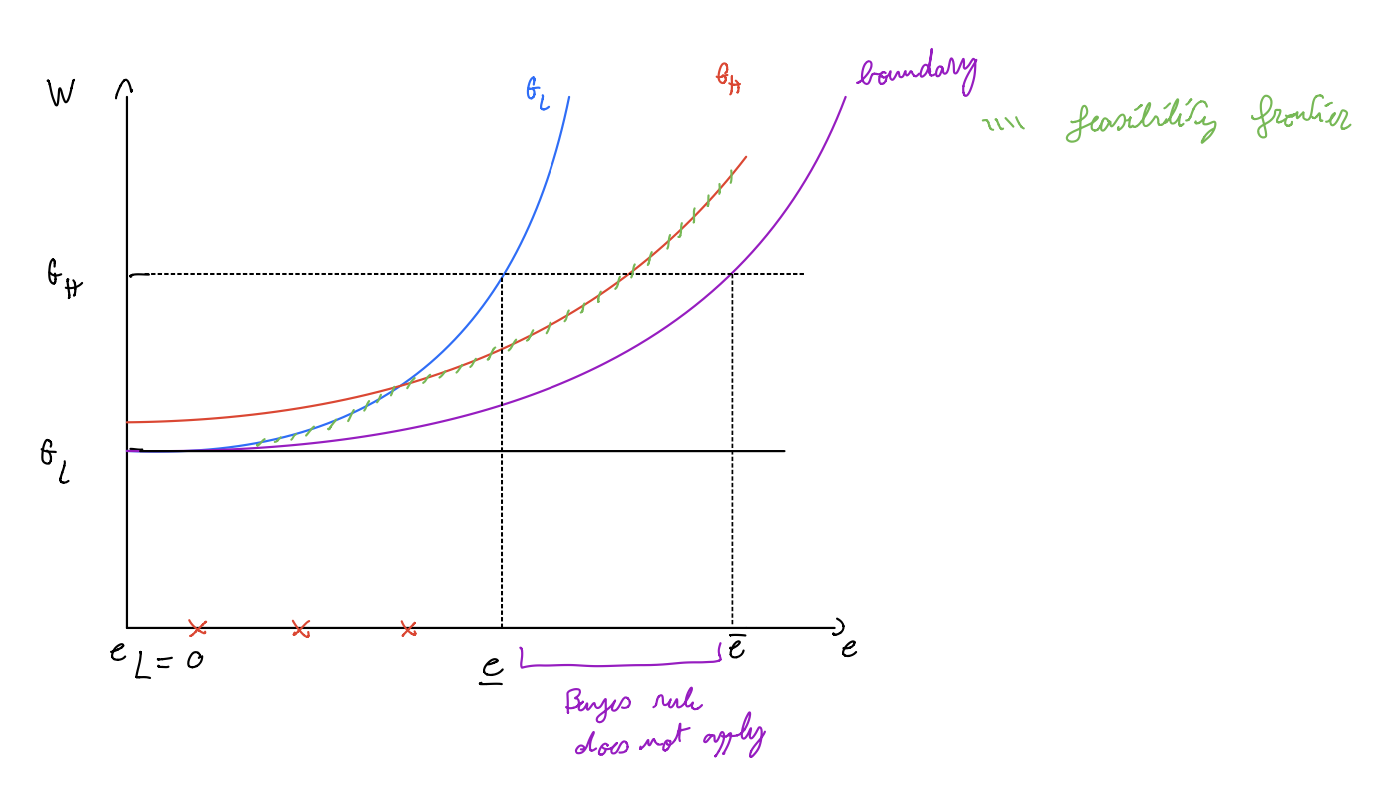
\includegraphics[width=0.9\linewidth]{sep_equilibria.png}
    \caption{Representation of the separating Equilibrium Case}
    \label{fig:enter-label}
\end{figure}
Assume $e(\theta_H)\neq e(\theta_L)$
    \begin{itemize}
        \item Step 1 - prove $e(\theta_L)$ = 0 : imagine $e(\theta_L)>0$, then if low worker picks $e(\theta_L)=0$ the firm will now assign a non negative probability of him being high types so the proposed wage will be at least as high as $\theta_L$ while reducing the cost (pure improvement). 
        \begin{equation}
            \theta_L-c(0,\theta_L) \geq \underbrace{\theta_H-c(e(\theta_H),\theta_L)}_{\text{utility if choose the same e as $\theta_H$}}
        \end{equation}
        \item Step 2 - finding $e(\theta_H)$ : we can easily establish the $e(\theta_H)$ with be above 0 (otherwise they would get $\theta_L$). 
        \begin{equation}
            \theta_H-c(e(\theta_H),\theta_H) > \theta_L-c(0,\theta_H)
        \end{equation}
        \item Step 3 : we now need to consider the case where a worker might wish to pick $e\notin [e(\theta_L),e(\theta_H)]$. To do this we must pick $\mu(e)$ low enough to have : (we could fix $\mu(e)=0$ arbitrarily for instance)
        \begin{equation}
        \begin{aligned}
            \theta_H - c(e(\theta_H),\theta_H) \geq w(e)-c(e,\theta_H)\\
            \theta_L - c(0,\theta_L)\geq w(e)-c(e,\theta_L)
        \end{aligned}
        \end{equation}
        \item Step 4 - additional conditionas on $(e(\theta_H))$: 
        \begin{enumerate}
            \item notice that if $\theta_L$ workers are indifferent between "no education | low wage" and (High education | high wage" then $\theta_H$ ones will stritly prefer having "High education | High wage" since they have a lesser cost of education due to the single crossing property.
            \begin{equation}
                \theta_L-c(0,\theta_L)=\theta_H-c(\underline{e},\theta_L)
            \end{equation}
            \item Similarly, if $\theta_H$ workers are indifferent between the two options, the inequality for $\theta_L$ workers will hold strictly (will always prefer not paying for education and getting $\theta_L$)\footnote{if $e(\theta_H)$ is already judged too expensive for high type, then it will be even more so for low types}
            \begin{equation}
                \theta_H-c(\bar{e},\theta_H)=\theta_L-c(0,\theta_H)
            \end{equation}
        \end{enumerate}
    \begin{simplebox}{Why Bayes rule does not apply when $e\in[\underline{e};\bar{e}]$}
   
These are off-path actions—actions that have zero probability of occurring in equilibrium. Since no worker is expected to choose an education level in between these two in a separating equilibrium, Bayes' rule cannot be applied to update beliefs based on such observations.

Without any equilibrium probability mass, the updating process is not well-defined, and the assignment of beliefs is indeterminate or arbitrary according to equilibrium refinements (like the Intuitive Criterion or the Divinity Criterion).
        
    \end{simplebox}
 \end{itemize}


\subsubsection{Solving for PBE : Pooling Equilibria}
\begin{figure}[H]
    \centering
    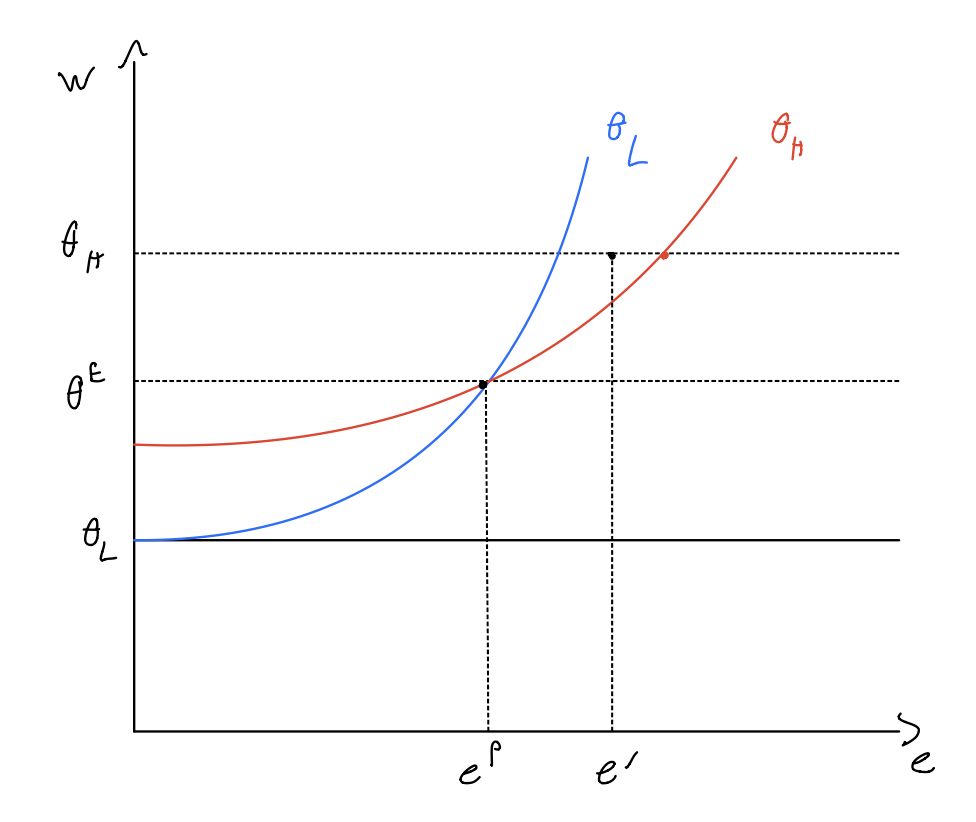
\includegraphics[width=0.6\linewidth]{pool_eq.png}
    \caption{Representation of the Pooling Equilibria}
    \label{fig:enter-label}
\end{figure}
Assume every worker chooses the same education level $e^P$ with probability 1. We define : with $\theta_E$ the expected productivity of a worker (similar to pooling wage)
\begin{equation}
\begin{aligned}
     &\text{Pooling wage : }w(e^P) = \lambda\theta_H+(1-\lambda)\theta_L\\
     &\text{Critical Education level : }\theta^E-c(\hat{e},\theta_L)=\theta_L-c(0,\theta_L)
\end{aligned}
\end{equation}
 the critical education level identifies the max education level a low-ability worker would be willing to acquire in a pooling equilibrium. Low worker will be indifferent between :
 \begin{itemize}
     \item Choosing $\hat{e}$ and receiving pooling wage $\theta_E$ (worker will never choose $e^P>\hat{e}$, otw would deviate to e=0) 
     \item choosing e=0 and receiving $\theta_L$
 \end{itemize}
 \textbf{Solving method : }
\begin{itemize}
    \item Step 1 ($e^P\leq\hat{e})$- prove that for any $e^P\in[0,\hat{e}]$ there is a pooling eq in which all workers choose $e^P$ for certain: 
    \begin{enumerate}
        \item suppose $\forall e\neq e^P,\mu(e)=0$ so that $w(e)=\theta_L<w(e^P)$ $\Rightarrow $if employer witness any education level $\neq \theta_P$ they will assume by default this is a $\theta_L$ worker !
        \item no one will want to choose $e>e^P$, besides $\theta_L$ workers will prefer $e^P$ by definition of $\hat{e}$\footnote{Proof: $c(e^P,\theta_L) \leq c(\hat{e},\theta_L)$ since education is costly and $e^P\leq\hat{e}$. Then $\theta_E - c(e^P,\theta_L) \geq \theta_E - c(e^b,\theta_L) = \theta_L - c(0,\theta_L)$ so it is not profitable to deviate to $e=0$ or to any $e\neq e^P$ (since deviation to 0 would have been the most profitable)}
        \item by the single crossing property, it will be the same for types $\theta_H$ (since education is relatively less costly for them)
    \end{enumerate}
    \item Step 2 (intuitive criterion check) : prove that in the job market signalling model, any pooling equilibrium fails the intuitive criterion. Here we can easily find an example graphically (we called it $e'$ on the graph) where the high type is made better off (places above his utility curve) by picking $e > e^P$
\end{itemize}
    \begin{simplebox}{The Intuitive Criterion }
        \textbf{Goal :} restricting beliefs to only include types that might reasonably deviate, the Intuitive Criterion often eliminates pooling equilibria in favor of separating equilibria in signaling games. \\
        Let $BR_2(T,a_1)$ denote the set of player 2's best responses if player 1 chose $a_1$ and player 2's beliefs have support in $T \subset \Theta$:  
            \begin{align}  
            BR_2(T,a_1) = \bigcup_{\mu \in \Delta(T)} \arg\max_{a_2 \in A_2} \sum_{\theta \in \Theta} u_2(a_1, a_2, \theta)\mu(\theta)
            \end{align}  
        \begin{definition}[Intuitive Criterion]  
                A Perfect Bayesian Equilibrium $s^*$ fails the intuitive criterion if there exists $a_1 \in A_1$, $\theta' \in \Theta$ and $J \subset \Theta$ such that:  
                \begin{align}  
                1.\ & u_1(s^*, \theta) > \max_{a_2 \in BR_2(\Theta, a_1)} u_1(a_1, a_2, \theta) \quad \forall \theta \in J \\  
                2.\ & u_1(s^*, \theta') < \min_{a_2 \in BR_2(\Theta \setminus J, a_1)} u_1(a_1, a_2, \theta')  
                \end{align}  
                where $BR_2(T, a_1)$ denotes the set of player 2's best responses if player 1 chose $a_1$ (an off equilibrium action) and player 2's beliefs have support in $T \subset \Theta$.  
            \end{definition}  
        \begin{itemize}
            \item The first inequality corresponds to the group J of types that will never want to deviate as their equilibrium payoff $u_1(s^*,\theta)$ $\Rightarrow$ \textbf{Types in J would never have played a1 since even if they could convince player 2 they were of a particular type they would do worse}
            \item The second inequality corresponds to the group of types, not included in J,  that would benefit from deviating to an off equilibrium action (equilibrium payoff is strictly less than the worse payoff they could get from deviating) $\Rightarrow$ \textbf{Type $\theta'$ definitely does better playing a1 rather than the equilibrium if she can convince player 2 that her type is not in J}
        \end{itemize}
         The Intuitive Criterion thus distinguishes between types that could potentially benefit from a deviation and those that definitely would not, eliminating equilibria that rely on implausible beliefs about which types might deviate.  \\
        \textbf{A concrete example :} 
        \begin{itemize}
            \item High types might benefit from deviating to high education if employers believed only high types would make this deviation
            \item Low types would never benefit from this deviation regardless of employer beliefs
            \item Therefore, the pooling equilibrium fails the Intuitive Criterion
        \end{itemize}
    \end{simplebox}

\subsection{General Solving method for PBE}
\subsubsection{Set-up}
Here we consider a two player signaling game where the first player can pick either 3 or 5 and player 2 can accept or decline the proposal made by player 1. The first player is either honest or dishonest (types)
\subsubsection{Finding Separating Equilibria}
\begin{itemize}
    \item Step 1 : decide on the equilibrium strategy played by each type of player 1 knowing both types can't play the same strategy. Note $\mu_3,\mu_5$ the belief function of player 2 knowing player 1 played 5 (3 respectively) before. Since we are considering a separating equilibria $\mu_5,\mu_3$ are either 0 or 1 (no intermediate probability), for instance : 
    \begin{equation}
    \begin{aligned}
        \mu_5 = P(\theta_H|5) = 1 
        \mu_3 = P_(\theta_H|3) = 0 
    \end{aligned}
    \end{equation}
    \item Step 2 : based on these strategies and probabilities, see how the game will unfold (check player 2's decisions at the end of each path taken by P1 at equilibrium)
    \item Step 3 : check whether the equilibrium path is optimal
    \item Step 4 : check if there are rational off-equilibrium deviations (look at outcomes if Player 1 player differently, for instance if the honest type player 3 in our above example)
\end{itemize}
\subsubsection{Finding Pooling Equilibria}
\begin{itemize}
    \item Step 1 : we decide on the equilibrium strategy that is played by both types, knowing both types will play the same strategy. Denote the $\mu_X$ for the strategy played as p and consider the other one to be determined arbitrarily (off the equilibrium path). For instance, if both the honest and dishonest type play 5, we note : 
    \begin{equation}
    \begin{aligned}
        &\mu_5 = p\\
        &\mu_3= arbitrary
    \end{aligned}
    \end{equation}
    \item Step 2 : look at expected conditional payoffs for player 2 as a function of p and $\mu_3$ (in our example). 
    \item Step 3 (indifference) : equate expected conditional payoffs that are on the same subgame (for instance $E(Accept|5) = E(Refuse|5)$) and find a cutoff value for $\mu_3$ $\Rightarrow$ enables us to determine how many potential values we must consider for $\mu_3$ to fully explore the problem
    \item Step 4 : For $\mu_3$ on either side of the cutoff value, check if there exists profitable deviations for each of the player 1 types. This gives us our first PBE.
    \item we note the PBE this way : if we consider the case $\mu_3<2/5$ with $2/5$ our cutoff value
    \begin{equation}
        PBE : \left\{(\text{path chosen by honest P1, path chosen by dishonest P1), (response of P2 to 5, response of P2 to 3), $\mu_5=p$,$\mu_3<2/5$}    \right\}
    \end{equation}
\end{itemize}
Vary the equilibrium strategy and the side of the cutoff value considered to capture all possible PBEs. 

\section{Session 9 : Incomplete information - Dynamic games }

\noindent \textbf{Two classes of models}
\begin{itemize}
    \item non verifiable information (cheap talke games) : actors can tell actual lies
    \item verifiable information : actors can only lie by omission
\end{itemize}

\subsection{Definitions}
\begin{itemize}
    \item Symmetric equilibrium : all player follow the same strategy in equilibrium
\end{itemize}

\subsection{The Cheap Talk Game}
\subsubsection{Set-Up}
\begin{itemize}
    \item 3 stage games : 
    \begin{enumerate}
        \item nature choose type of $P_1$(sender) from distribution p
        \item $P_1$ observes $\theta$ and chooses $m\in M$ (message he wishes to send)
        \item $P_2$(receiver) observes m and chooses $a\in A$
    \end{enumerate}
\end{itemize}
\subsubsection{The non separating equilibrias problem}
Communication difficulty : credible communication\footnote{communication that actually conveys information about the state of world} is complicated if : 1) all types of senders have perfectly aligned preferences (all receiver will play the same way so no additional info) , 2) all types of senders have perfectly opposed preferences (too much variation, so the receiver just won't listen to the messages)
$\Rightarrow$ separating equilibria in cheap talk games do not always exist in these settings (depends on receiver payoffs\footnote{see slide 8 vs slide 10}) !
\begin{Proof}
    \begin{itemize}
        \item Aligned preferences case : types are fully revealed by the message. So all types can get more by sending the same message as the type who gets the most out of his message (profitable deviation from separating strategy exists)
        \item Opposed preferences case  : same intuition except both type will wish to switch messages with each other (instead of all turning to the same most profitable message)
    \end{itemize}
\end{Proof}
\subsubsection{General model set-up}
\begin{itemize}
    \item types : $\theta\sim U[0,1]$
    \item P2 has actions denoted $a\in \mathcal{R}$ and payoff $u_2(a,\theta)=-(a-\theta)^2$
    \item P1 has payoff $u_1(a,\theta)=-(a-\theta-c)^2$
    \item optimal choice differs across players ($a=\theta$ vs $a=\theta+c$)
\end{itemize}
\textbf{Babbling equilibrium}
\begin{itemize}
    \item $P_1$ send m no matter $\theta$ (no info conveyed so no bayesian updating) so $P_2$ assigns equal probability to all values of $\theta$ regardless of m (since $\theta$ follows uniform distribution). THen $P_2$ sets action $a=E[\theta]=1/2$
\end{itemize}
\textbf{Two message equilibrium}
\begin{itemize}
    \item $P_1$ sends $m_1$ or $m_2$ and we impose $a(m_1)<a(m_2)$ (message conveys information)
    \item step 1 - show $P_1$ adopts a threshold strategy with $\theta^*$ : just show the incremental gain for player 1 $payoff(m_2)-payoff(m_1)$ is increasing in $\theta$ (if pick $m_2$ for a $\theta^*$ then you will wish to pick the same message for any $\theta>\theta^*$)
    \item step 2 - find the equilibrium values of $a(m_1),a(m_2)$ : 
    \begin{enumerate}
        \item $P_2$ set : $a(m)=E[\theta|m]$
        \item when $P_2$ receives $m_1$ he knows $\theta\sim[0,\theta^*]$ so $a(m_1)=E[\theta|m_1]=\frac{\theta^*}{2}$
        \item same reasoning for $m_2$ gives us : $a(m_2) = E[\theta|m_2]=\frac{1+\theta^*}{2}$
        \item indifference condition : we find the $P_1$ cutoff value $\theta^*$ using the fact that at $\theta^*$ we must have\footnote{be careful since when taking the square root we have absolute values so it's better to directly multiply the left hand side by $(-1)^2$ to ensure we have  directly a positive term when taking the root}
        \begin{equation}
            u_2(a(m_1),\theta^*)=u_2(a(m_2),\theta^*)
        \end{equation}
        \item we know $\theta^*>0$ which gives us a condition on c
    \end{enumerate}
\end{itemize}
\textbf{Three message equilibrium}
\begin{itemize}
    \item now : $[0,\theta_1)$ choose $m_1$, ($\theta_1,\theta_2$) choose $m_2$ and the rest choose $m_3$
    \item we use exactly the same reasoning except we now have two indifference conditions 
    \item look at the condition on c and notice that the threshold for the three message equilibrium is lower than for the two message one, so can have both in this situation. (threshold fgives us the maximum number we can communicate given a certain value of c)
\end{itemize}


\subsection{The War of attrition game}
\subsubsection{Set-Up : }
\begin{itemize}
    \item 2 firms fight to be the only one in a market and get a prize of $v>1$
    \item As long as they are both in the market, they make a loss of 1 per period (cost of fighting)
    \item payoff of one of the firms leaving at t : 1)for the loss equality notice we have a finite geometric series with a=1 and r=$\delta$\footnote{To see more about this formula : \hyperlink{https://en.wikipedia.org/wiki/Geometric_series}{About geometric series}}2) for total utility note we have a one time benefit of 1 (not a perpetuity)
    \begin{equation}
    \begin{aligned}
       \text{Loss until period t : } L(t) = -1-\delta-\delta^2...-\delta^{t-1} = -\sum_{k=0}^{t-1}\delta^k=\frac{1-\delta^t}{1-\delta}\\
       \text{Total utility for firm which stays : } F(t)=L(t)+\delta^tv
    \end{aligned}
    \end{equation}
\end{itemize}
\subsubsection{solving for equilibrium}
\textbf{Equilibrias in discrete time : }
\begin{itemize}
    \item asymmetric equilibria : $P_1$ never stops and $P_2$ always stops (so stops immediately basically)
    \item mixed strategy equilibria : both players play the same strategy "if other has not stopped before t, I stop at t with probability p"
    \begin{enumerate}
        \item We wish to find p such that each firm i is indifferent between stopping at t or t+1
        \item to get it just solve for p using this indifference equality : 
        \begin{equation}
            \underbrace{L(t)}_{\text{cost of exiting at t}} = \underbrace{\underbrace{pF(t)}_{\substack{\text{firm j stops}\\\text{with proba p}}}+(1-p)L(t+1)}_{\text{utility of staying in period t+1}}
        \end{equation}
    \end{enumerate}
\end{itemize}
\textbf{Equilibrias in countinuous time}
\begin{itemize}
    \item modeling continuous time: consider period of lenght $\delta$ and make them tend towards 0. We denote : $n=t/\Delta$ the number of periods between 0 and t. 
    \item Step 1 :  we find the equilibrium probability of stopping $p^*$ through : 
    \begin{equation}
        \underbrace{p^*v}_{\text{MB of continuing}}=\underbrace{(1-p^*)\Delta}_{\text{MC of continuing}}
    \end{equation}
    \item Step 2 - find the probability that a player does not stop before t : 1) Write down probability of not stopping for n periods, 2) Substitute n by its expression, 3) Rewrite it with an exponential and use a taylor approximation for the ln function (possible given $\Delta$ small)
    \begin{equation}
    \begin{aligned}
        &1-G(t)=(1-p^*)^ n \approx e^{-t/v}\\
        &\text{with G(t) the probability of stopping before t (it is a distribution) }
    \end{aligned}
    \end{equation}
    \item Step 3 : rewrite the discount factor as a function of the interest rate r 
    \begin{equation}
        \delta^t=(e^{-r})^t
    \end{equation}
    \item Step 4 : rewrite the loss function $L(t)$ as an integral of the discount factor between 0,t
    \begin{equation}
        L(t) = \int_0^te^{-rs}ds = \frac{1}{r}[1-e^{-rt}]
    \end{equation}
    \item Step 5 : we write $F(t)$ using the same formula that we used for discrete time 
    \begin{equation}
        F(t) = [L(t)+e^{-rt}v]
    \end{equation}
    \item Step 6 - write the expected profits of stopping at time T : we integrate over t given a density g(t)\footnote{PDF of the opponent's stopping time} for stopping at a time t\footnote{we account for the fact that at each period, the other firm has a non null probability of exiting}
    \begin{equation}
        E(\text{profits of stopping at T})=\underbrace{\int_0^TF(t)g(t)dt}_{\text{E(payoff) if opponent stop at $t\leq T$}}+\underbrace{\int_T^{+\infty}L(T)g(t)dt}_{\text{E(payoff) if opponents stop at t>T}}
    \end{equation}
    \item to visualize it more easily, you may view this as a weighted sum of all possible outcomes with a given weight g(t)dt for each outcome. (we sum over the full distribution of g(t)
    \item Step 7 - derive expected profits with respect to T (use Leibniz rule) and set it to 0 (players are indifferent between when to stop) to get the hazard rate $\frac{g(T)}{1-G(T)}$
    \item The hazard rate measures the instantaneous probability of the opponent stopping at time T, given they have survived up to T
\end{itemize}


\end{document}


